\documentclass{article} % For LaTeX2e
\usepackage{nips13submit_e,times}
\usepackage{hyperref}
\usepackage{url}
\usepackage{amsmath}
\usepackage{graphicx}
\usepackage{float}
\usepackage{caption}
\usepackage{subcaption}
\floatplacement{figure}{H}
%\documentstyle[nips13submit_09,times,art10]{article} % For LaTeX 2.09


\title{Fast Support Vector Data Descriptions for Novelty Detection\\ Project Report\thanks{As a part of the course Kernel Methods for Pattern Analysis - CS6011 Jan - May 2015}}



\author{
Aravind Sankar \\
CS11B033 \\
Department of Computer Science\\
IIT Madras\\
\texttt{aravindsankar28@gmail.com} \\
\And
Adit Krishnan \\
CS11B063\\
Department of Computer Science\\
IIT Madras\\
\texttt{adit101293@gmail.com} \\
}

% The \author macro works with any number of authors. There are two commands
% used to separate the names and addresses of multiple authors: \And and \AND.
%
% Using \And between authors leaves it to \LaTeX{} to determine where to break
% the lines. Using \AND forces a linebreak at that point. So, if \LaTeX{}
% puts 3 of 4 authors names on the first line, and the last on the second
% line, try using \AND instead of \And before the third author name.

\newcommand{\fix}{\marginpar{FIX}}
\newcommand{\new}{\marginpar{NEW}}

\nipsfinalcopy % Uncomment for camera-ready version

\begin{document}


\maketitle

\begin{abstract}
The abstract paragraph should be indented 1/2~inch (3~picas) on both left and
right-hand margins. Use 10~point type, with a vertical spacing of 11~points.
The word \textbf{Abstract} must be centered, bold, and in point size 12. Two
line spaces precede the abstract. The abstract must be limited to one
paragraph.
\end{abstract}




\section{Brief Summary}
\subsection{Introduction}

In this paper, the authors address the common well-studied problem of Novelty Detection. In this task, we have a 2-class problem denoted by the normal and abnormal class points, where the number of points of abnormal class is lesser than that of the normal class. We note that this problem is different from the traditional classification problem in that only points of the normal class are used for the purpose of training, essentially a One-Class classification problem.  \\[10pt]

The Support Vector Data Description (SVDD)[1]  is an important and popular technique which has been used to solve the problem of Novelty Detection. In short, SVDD tries to construct a soft minimal hypersphere enclosing the points of the target class (normal) in the kernel feature space ($\phi$). This hypersphere boundary in the kernel feature space is used for prediction to identify the outlier points (novel data). It can also be shown that the decision boundary between the 2 classes is a hyperplane in the kernel feature space if a normalized kernel function is used. SVDD like any other SVM, has a prediction time complexity linear in the number of support vectors ($N_s$) because $N_s$ evaluations of the kernel function is required for predicting the label of an unseen data point. \\[10pt]

The authors attempt to address this key issue in this paper by proposing Fast SVDD (F-SVDD) [2] which replaces the kernel expansion (of $N_s$ terms) in the decision function with just 1 term. This is achieved by first looking for a vector (called agent of the center) in the $\phi$-space whose preimage $\hat{x}$ exists in the $x$-space. Then, they express the sphere center $a_{\phi}$ as a scalar multiple of this vector in the $\phi$-space. Now, it can be seen the decision function involves only one kernel function between $\hat{x}$ and any unseen data point $x$. This means that the prediction time complexity is constant, irrespective of the size of the training dataset and the number of support vectors. The authors also propose an efficient method for solving the preimage problem, which is non-iterative and faster than the existing techniques. The approaches used to solve these problems will be explained in the further sections.


\subsection{SVDD and some properties}
In this section, we introduce the SVDD problem definition for the purpose of notation. The optimization problem that we solve for involves $a_\phi$ (center of the sphere), $\left\lbrace \xi_i \right\rbrace_{i=1}^N$ (slacks) and $R$ (radius of the hypersphere) as the optimization variables while $C$ is a user specified cost parameter. We assume that we have a training dataset $D = \left\lbrace x_i \right\rbrace_{i=1}^N$.
The primal and dual problems are shown below :
\\[10pt]

\textbf{Primal problem (with constraints) :}
\begin{equation}
\begin{split}
\text{min} \; R^2 + C \sum\limits_{i=1}^N \xi_i \\
\text{subject to}\\
||\phi(x_i) - a_{\phi}||^2  \leq R^2 + \xi_i \\
\xi_i \geq 0 \;\; \forall i = 1,...N
\end{split}
\end{equation}

\textbf{Dual problem:}

\begin{equation}
\begin{split}
\text{max}\; 1 - \sum\limits_{i=1}^N \sum\limits_{j=1}^N \alpha_i \alpha_j K(x_i,x_j) \\
\text{subject to}  \\
\sum\limits_{i = 1}^N \alpha_i  = 1  \\
0 \leq \alpha_i \leq C \;\; \forall  i = 1,...,N.  
\end{split}
\end{equation}

As usual, the lagrange multipliers $\left\lbrace \alpha_i \right\rbrace_{i=1}^N$ are associated with the primal constraint involving $\xi_i$'s.
Here, the discriminant function $g(x)$ is given by :

\[ g(x) = ||\phi(x_i) - a_{\phi}||^2 - R^2 = c - 2 \sum\limits_{i=1}^{N_s}\alpha_i K(x,x_i) \]
where $c$ is a constant. \\[10pt]


The sphere center $a_\phi$ is given by :

\[ a_\phi  = \sum\limits_{i=1}^{N} \alpha_i \phi(x_i) = \sum\limits_{i=1}^{N_s} \alpha_i \phi(x_i)\]

We also compute $||a_\phi||$ as it will be used later, 
\begin{equation} \label{norm}
||a_\phi||^2 = ||\sum\limits_{i=1}^{N_s} \alpha_i \phi(x_i) ||^2  = \alpha^T K \alpha
\end{equation}

where $K$ is the kernel gram matrix. \\[10pt]


Let the soft minimal hypersphere (constructed by SVDD over the training points) be denoted as $B_S$. We assume the use of a gaussian kernel function (can  be extended for any normalized kernel also) so that $K(x,x) = 1$. So, all points $\phi(x)$ lie on a unit hypersphere (centered at origin $O_\phi$) in the kernel feature space, denoted by $B_\phi$. This leads to interesting geometrical properties in the kernel feature space. One main property is mentioned below : \\[10pt]

\textbf{Property :} The center $a_\phi$ of the SVDD hypersphere $B_S$ must lie inside the unit hypersphere $B_{\phi}$. \\[10pt]


This property shows that the exact preimage of $a_\phi$ in the x-space does not exist. This means that, either only an approximate preimage can be found, or a different way needs to be found. F-SVDD does this by identifying the \textit{agent} of the center whose pre-image exists in the x-space. The following sections explain the process of finding the agent and the corresponding preimage.


\subsection{Fast SVDD}
The main objective of F-SVDD is to improve classification speed by reducing the number of computations at prediction time. By the above property, the preimage of the center $a_\phi$ does not exist. This algorithm  
first defines the agent of the center.

\subsubsection{Agent of the center}

Let the agent of the center be denoted by $\Psi_a$ (in the kernel feature space). We want $\Psi_a$ to have a pre-image $\hat{x}$ in the x-space.  This directly implies that $\Psi_a$ should lie on the unit hypersphere  $B_{\phi}$ centered at Origin in the kernel feature space. This gives us  

\begin{equation}\label{norm1}
||\psi_a|| = 1 
\end{equation}

$\Psi_a$ is identified as the point closest to $a_\phi$ that lies on $B_{\phi}$. This point is obtained by  extending $a_\phi$ to intersect $B_\phi$. obviously is in the direction of $a_\phi$.
Thus, we can express $\Psi_a$ as :

\begin{equation}
\begin{split}
\Psi_a &= \gamma a_\phi \\\\
&\text{where } \gamma  \text{ is a scalar.} \\ \\
||\Psi_a|| &= \gamma ||a_\phi||  \\
\gamma &= \frac{1}{||a_\phi||}  \text{  (Using  \ref{norm1})} \\ 
\gamma &= \frac{1}{\sqrt{\alpha^T K \alpha}} \text{  (Using  \ref{norm})} 
\end{split}
\end{equation}


We also note that $\gamma >1$ as $||a_\phi|| < 1$.

This shows us that if we are able to obtain the preimage of the agent, the computation of our discriminant function reduces to just 1 term, which involves just $\hat{x}$. In the next section, we describe how the pre-image is computed for the agent.



\subsubsection{Preimage of the agent :}

Formally, we define the preimage problem as, given a feature vector $\psi$ in the kernel feature space, find $\hat{x} \in \mathbf{R}^d $ (x-space) such that $\psi = \phi(x)$.
The preimage $\hat{x}$ is found by solving the problem :

\[ \hat{x} = \min_{\hat{x}} ||\Psi_a - \phi(\hat{x}) ||^2   \]

It can shown that solving this problem is equivalent to finding the approximate preimage of $a_\phi$, i.e.

\[ \min \rho = ||a_\phi - \phi(\hat{x}) ||^2 \]


To minimize $\rho$, we set the derivative of the objective function ($\rho$) to 0 and we obtain : 

\[ \hat{x} = \frac{\sum\limits_{i=1}^N \alpha_i K(\hat{x},x_i)x_i}{\sum\limits_{i=1}^N K(\hat{x},x_i)} \]

We see that $\hat{x}$ appears on both sides of the above equation. One of the ways to solve such an equation is shown below :
\subsubsection*{Fixed point iteration}

Fixed point iteration is an existing technique for computing fixed points of iterated functions.
It can be used here to solve for $\hat{x}$. Initially, $\hat{x}$ is set to a random value $x_0$ and then an iterative procedure is followed to get the final fixed value of $\hat{x}$. The equation below shows the procedure :

\[ \hat{x}_{t+1} = \frac{\sum\limits_{i=1}^N  \alpha_i  K(\hat{x}_t,x_i) x_i}{\sum\limits_{i=1}^N  \alpha_i K(\hat{x}_t,x_i)} \]

Though the above method will converge to the optimal value of $\hat{x}$ (in general), it faces the problems of local minima and it also requires multiple initial guesses for $\hat{x}$ which leads to an increase in computation time. In order to solve these issues, the authors have proposed a direct pre-image finding method, which is given below :


\subsubsection*{Direct Method} 

In this technique, some simple properties of kernel functions are used to arrive at a closed form expression for $\hat{x}$.
\[ \hat{x} = \frac{\sum\limits_{i=1}^N \sum\limits_{j=1}^N \alpha_i \alpha_j K(x_i,x_j) x_i}{\sum\limits_{i=1}^N \sum\limits_{j=1}^N \alpha_i \alpha_j K(x_i,x_j)} \]
We can clearly see that the problems faced by the fixed point iteration method have been eliminated here.	

\subsubsection{Discriminant function}
Finally, the discriminant function $g(x)$ is given by 

\begin{equation} \label{disc}
\begin{split}
g(x) &= || \phi(x) - a_\phi||^2 - R^2 = ||\phi(x) - \frac{\phi(\hat{x})}{\gamma} || - R^2 \\
 &=   c' - \frac{2}{\gamma} K(x,\hat{x}) \\ 
 & \text{where}\;  c' = 1- R^2 + 1/\gamma^2 \; \text{is a constant}.
\end{split}
\end{equation}
Thus, we can see that the $g(x)$ has only one kernel function term, which makes the prediction time complexity a constant. 

\section{Experiments}
In this section, we describe the experiments that were performed to compare the performance of F-SVDD with C-SVDD. Specifically, we compare F-SVDD - 1 (direct preimage finding method), F-SVDD - 2 (fixed point iteration method) and C-SVDD (basic SVDD formulation) for the performance in terms of generalization performance (accuracy) and classification speed (training and testing). In addition to this, we also compare the generalization performance against a non-kernel method which is that of a Multi-Layer Feed Forward Neural Network (MLFFNN) [3]. MATLAB was used to implement all of the three SVDD algorithms, specifically using the optimization toolbox. MLFFNN was implemented using the default MATLAB toolbox. 

We use 2 real world datasets obtained from the UCI ML\footnote{http://archive.ics.uci.edu/ml/} repository and one synthetic dataset (from our assignment) for our evaluation. We also use another synthetic dataset to illustrate the differences between F-SVDD and C-SVDD. \\[5pt]

All the experiments were performed on a system with Intel 2.3 GHz i5 processor and 6 GB main memory. \\[5pt]


In all our experiments (expect overlapping dataset) involving SVDD and associated algorithms, the best values of the parameters $C$ and $\sigma$ were found by performing 10-fold cross validation. These values were obtained by performing cross validation for the C-SVDD algorithm. For maintaining fairness of results, the same values of $C$ and $\sigma$ were used for the F-SVDD algorithms also. For the MLFFNN, we performed cross-validation to estimate the number of nodes in the hidden layer. \\[5pt]

\textbf{(Check this once and decide where to add it )}
In the paper, it has been mentioned that all of the training points are used as support vectors for C-SVDD, i.e. they do not perform a thresholding on the lagrange multipliers obtained due to precision issues. This could be one of the reasons why the testing times reported for C-SVDD in the paper are quite high in comparison to the F-SVDD method.



\textbf{Evaluation metric :}

The metric used for evaluating the generalization performance is  TAER (Total Average Error Rate) given by :
\[ \texttt{TAER} = \frac{\texttt{Number of misclassified points}}{\texttt{Total number of points}} \]

The values of TAER reported in the results section are the average values obtained over 50 random samples of training data (the rest of the points used for testing). 

We also evaluate the most important objective of this paper, which is the classification speed. We report both the training and testing times for each of the SVDD algorithms.

In the following subsections, we analyze the results obtained on each of the three datasets. \\[10pt]



\subsection{Overlapping classes dataset :} This is the same dataset that was used in our assignments. We use this for visualization and interpreting since it is 2 dimensional. In this dataset, we have 4 classes which are overlapping and hence linearly non-separable. So, a 100 \% accuracy cannot be expected for any classification/ novelty detection task on this dataset.
The scatter plot of the dataset is shown below :

\begin{figure}
  \centering
  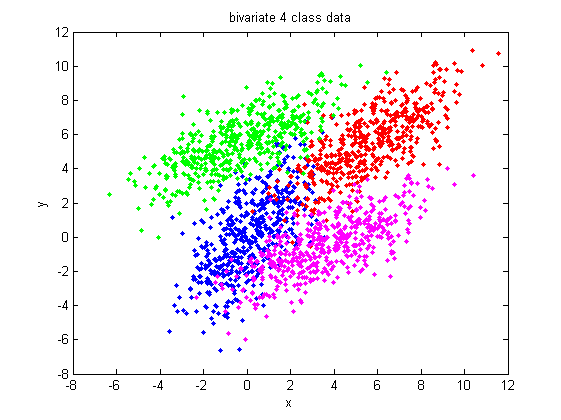
\includegraphics[width=\linewidth]{../Code/overlapping/svdd/data}
  \caption{Overlapping classes dataset with 4 classes}
\end{figure}

The above plot shows the un-normalized dataset, while we have used the min-max normalization to reduce the  range of each coordinate to $[0,1]$. 

For the task of Novelty detection , we need to define our target and outlier class points. So, we perform 4 experiments where in $\text{experiment}_{i}$ points of class $i$ are taken as the target (or normal) points, while the rest are considered as outliers. The size of training set was 250, while the sizes of validation and test sets were 600 and 400 respectively.

In this case, we are given explicit validation and test datasets. So, we find out the best values of $C$ and $\sigma$ only over the given validation set. The best value of $\sigma$ obtained was 0.3371. Also, the value of $C$ was estimated for each of the 4 experiments and the range of values of $C$ obtained was from 0.02 to 0.04.
The performance (TAER) obtained for each of the 4 experiments is shown below : \\[5pt]
\begin{table}[H]
\begin{center}
\caption{Comparison of Average Error rates on Overlapping classes dataset}
\begin{tabular}{|c|c|c|c|c|c|}
\hline
Target class & Evaluation set & C-SVDD & F-SVDD-1 & F-SVDD-2 & MLFFNN \\ \hline
 1 & Train & 0.1240 & 0.1480 & 0.1360 & . \\ 
 (N = 250) & Validation & 0.1117 & 0.1750 & 0.1733 &  \\ 
 & Test &  0.1475 & 0.1925 &  0.1925 & . \\ \hline
 
 2 & Train & 0.1160 & 0.1640 & 0.1640 & . \\ 
  (N = 250)& Validation &  0.1117  &  0.0867 &  0.0817 & . \\ 
 & Test &  0.1117  &  0.0800 & 0.0800  & . \\ \hline
 
 
 3 & Train & 0.1880 & 0.2080  & 0.2080 & . \\ 
 (N = 250) & Validation & 0.0817 & 0.1100 &  0.1100 & . \\ 
 & Test &  0.0875 &  0.1200 & 0.1200  & . \\ \hline
 
 
 4 & Train & 0.1040 & 0.1520 &  0.1760 & . \\ 
 (N = 250) & Validation &  0.0467 & 0.1217 & 0.1250 & . \\ 
 & Test & 0.0500 &  0.1450 &  0.1525 & . \\ \hline
 
& Average test error  &  0.0992 &  0.1344 & 0.1363 &. \\ \hline

\end{tabular} \\[10pt]
\end{center}

\end{table}

The decision region plots obtained for C-SVDD and F-SVDD for each of the 4 classes are shown below :

\begin{figure}[H]
\begin{subfigure}{.5\textwidth}
  \centering
  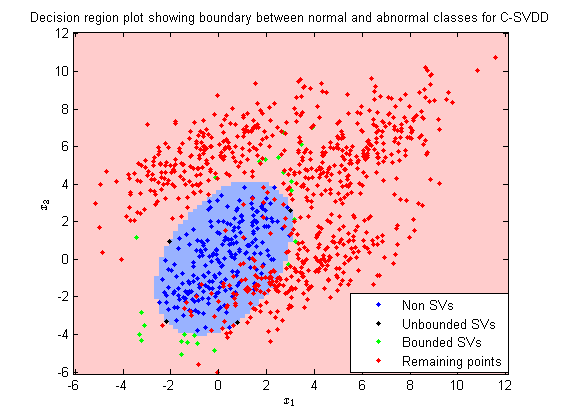
\includegraphics[width=\linewidth]{../Code/overlapping/svdd/decn_1}
\caption{C-SVDD} 
\end{subfigure}%
\begin{subfigure}{.5\textwidth}
  \centering
  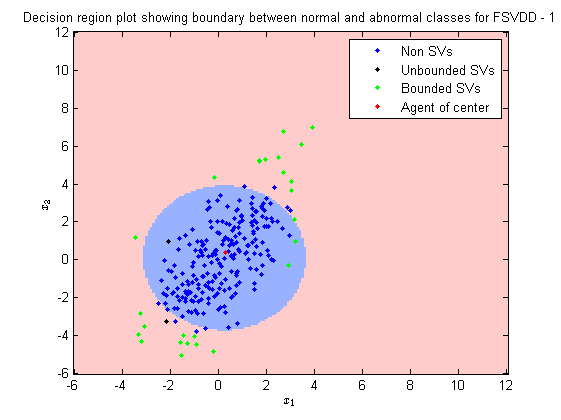
\includegraphics[width=\linewidth]{../Code/overlapping/fsvdd/decn_1}
\caption{F-SVDD} 
\end{subfigure}
\caption{Decision region plot with class-1 points as target class} 
\end{figure}


\begin{figure}[H]
\begin{subfigure}{.5\textwidth}
  \centering
  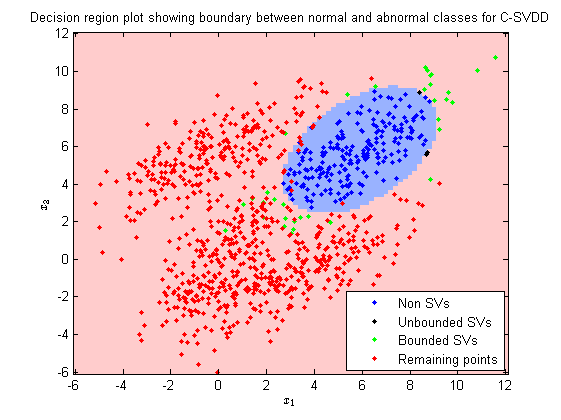
\includegraphics[width=\linewidth]{../Code/overlapping/svdd/decn_2}
\caption{C-SVDD} 
\end{subfigure}%
\begin{subfigure}{.5\textwidth}
  \centering
  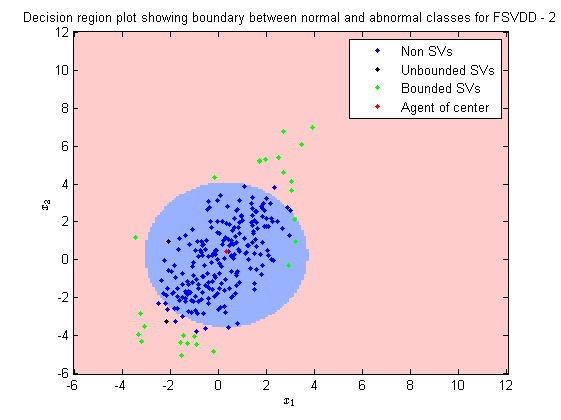
\includegraphics[width=\linewidth]{../Code/overlapping/fsvdd/decn_2}
\caption{F-SVDD} 
\end{subfigure}
\caption{Decision region plot with class-2 points as target class} 
\end{figure}



\begin{figure}[H]
\begin{subfigure}{.5\textwidth}
  \centering
  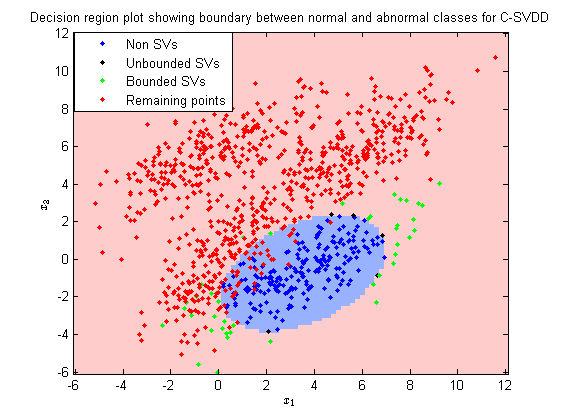
\includegraphics[width=\linewidth]{../Code/overlapping/svdd/decn_3}
\caption{C-SVDD} 
\end{subfigure}%
\begin{subfigure}{.5\textwidth}
  \centering
  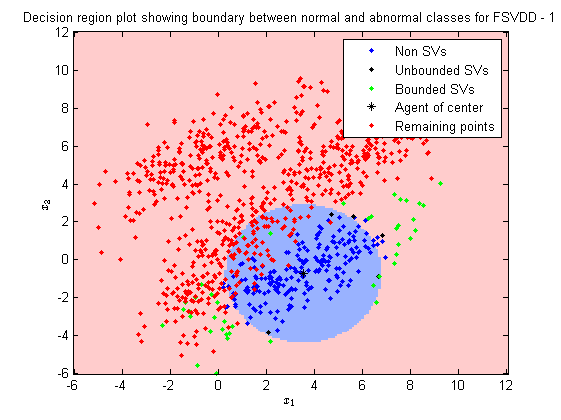
\includegraphics[width=\linewidth]{../Code/overlapping/fsvdd/decn_3}
\caption{F-SVDD} 
\end{subfigure}
\caption{Decision region plot with class-3 points as target class} 
\end{figure}



\begin{figure}[H]
\begin{subfigure}{.5\textwidth}
  \centering
  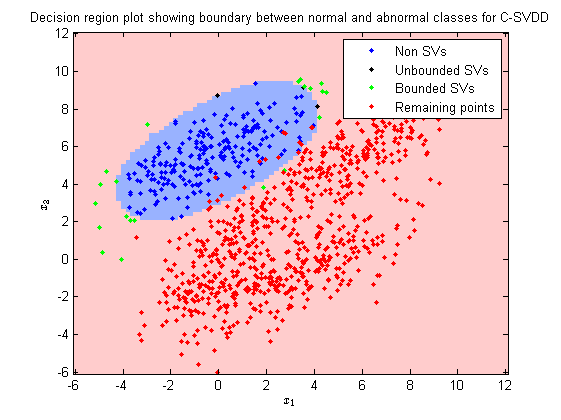
\includegraphics[width=\linewidth]{../Code/overlapping/svdd/decn_4}
\caption{C-SVDD} 
\end{subfigure}%
\begin{subfigure}{.5\textwidth}
  \centering
  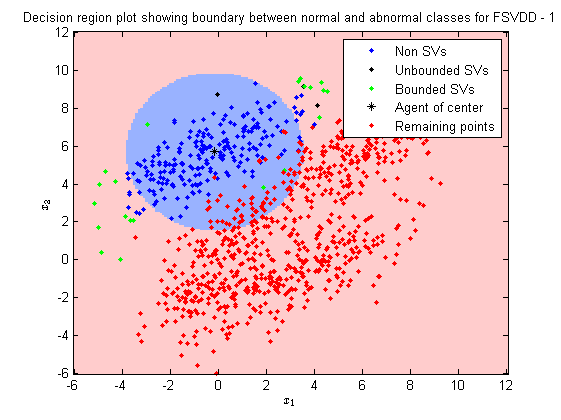
\includegraphics[width=\linewidth]{../Code/overlapping/fsvdd/decn_4}
\caption{F-SVDD} 
\end{subfigure}
\caption{Decision region plot with class-4 points as target class} 
\end{figure}

\textbf{Observations :}
\begin{enumerate}
\item We observe that the performance of F-SVDD  (both 1 and 2) is slightly inferior in comparison to that of C-SVDD. C-SVDD outperforms F-SVDD-1 by 3.5 \% on an average. This is because of the nature of the decision surfaces obtained using F-SVDD i.e  spherical in the x-space (will be explained later).

\item FSVDD-1 and FSVDD-2 perform very similarly in most of the cases and the difference in their average error rates is 0.0019 ~ 0.19 \% which is negligible. This is because, the $\hat{x}$ found by Fixed point iteration was very close to the one found by direct method. As the dataset is quite simple, the effect of different starting points did not play a role here.

\item The total error rate for class 1 was observed to be more than that of the other classes, for both the algorithms. This is clearly because of the points of this class have more overlap with the other class points. The error rates observed for the other class points were very similar.

\item The agent of the center $\hat{x}$ found by F-SVDD is also marked in the decision region plot, denoted by a black cross. It is the center of the spherical decision surface that we obtain in the x-space.

\end{enumerate}


The running times that were observed for each of the algorithms are shown below :
\begin{table}[H]
\begin{center}
\caption{Running time (in seconds) comparison for Overlapping classes dataset}
\begin{tabular}{|c|c|c|c|c|c|c|}
\hline
Target class & \multicolumn{2}{|c|}{C-SVDD} & \multicolumn{2}{|c|}{F-SVDD-1} & \multicolumn{2}{|c|}{FSVDD-2}  \\ \hline
& Training & Testing & Training & Testing & Training & Testing \\ \hline
1 & 0.3351 & 0.6312 & 0.3744  & 0.0187 & 1.0764 & 0.0156 \\ \hline
2 & 0.3551 & 0.7176 & 0.3588 & 0.0187 & 1.1232 & 0.0094 \\ \hline
3 & 0.3414 & 0.7722 & 0.3476 & 0.0171 & 1.4881 & 0.0094 \\ \hline
4 & 0.3120 & 0.7753 & 0.3744 & 0.0187 & 1.4661 &  0.0094 \\ \hline

\end{tabular} \\[5pt]
\end{center}
\end{table}


\textbf{Observations :}
\begin{enumerate}
\item The training time for F-SVDD-1 was found be higher than that of C-SVDD, which is because of the additional computation that is required for the computation of the agent of the center $\hat{x}$. But, we note that the difference in time taken is very less on an average.

\item On the contrary, the F-SVDD-2 takes abound 1.28 seconds on an average for training. This is much higher than the other two algorithms and has a lot more variation in the times for each of the classes. The excess time is due to the fact that the fixed point method requires a lot of iterations to converge.

\item The testing time for C-SVDD is found to be quite high due to the $N_s$ computations for the predicting of an unseen data point. In comparison, we observe that the testing time for F-SVDD-1 and 2 are negligible, as they involve only 1 computation for a new point. This shows the tremendous increase in classification speed in the F-SVDD algorithms.
\end{enumerate}

 
\subsection{Iris Dataset :} \footnote{https://archive.ics.uci.edu/ml/datasets/Iris}
This is a well known pattern recognition data set containing 3 classes of 50 instances each. This dataset is 4 dimensional with one linearly separable class while the other 2 overlap. Class 1 can be separated well from the other 2 classes. The dataset has 150 points in total, containing 50 points in each class.
The scatter plot of the dataset is shown below illustrates the separability when projected on the petal dimensions.




\begin{figure}[H]
\begin{subfigure}{.5\textwidth}
  \centering
  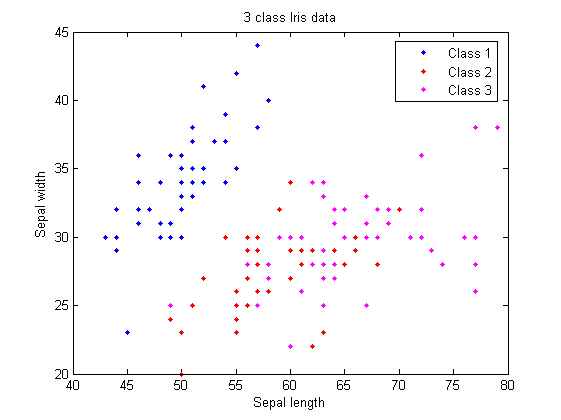
\includegraphics[width=\linewidth]{../Code/FisherIris/svdd/iris_1}
\caption{Scatter plot w.r.t Sepal width and length} 
\end{subfigure}%
\begin{subfigure}{.5\textwidth}
  \centering
  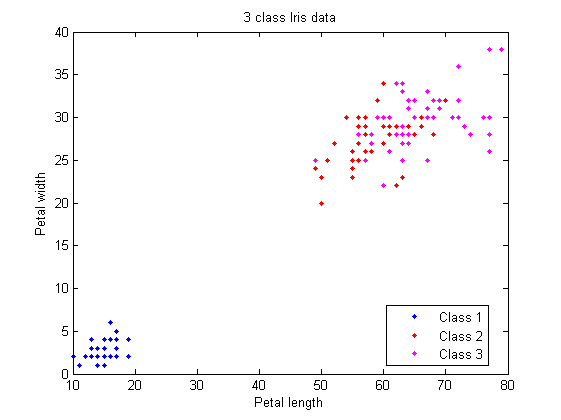
\includegraphics[width=\linewidth]{../Code/FisherIris/svdd/iris_2}
\caption{Scatter plot w.r.t Petal width and length}  
\end{subfigure}
\caption{Scatter plot of the Fisher Iris dataset}
\end{figure}

For the task of Novelty detection , we performed 3 sets of experiments considering each of the three classes as the target class and the rest of the points as outliers. For the purpose of discussion, let us choose class 1 as the target class. We choose 25 points of class 1 to train, and divide the rest into validation and test sets. The best values of $C$ and $\sigma$ obtained were $C = 0.4$ and $\sigma = 22.3$. 

...add more content here ...

The performance of the 3 algorithms on this dataset are shown below :


\begin{table}[H]
\begin{center}
\caption{Comparison of Average Error rates on Fisher dataset}
\begin{tabular}{|c|c|c|c|c|}
\hline
Target class & C-SVDD & F-SVDD-1 & F-SVDD-2 & MLFFNN \\ \hline
1 ($N_{train} = 25$) &  0.0224  & 0.0275  & 0.0296  &. \\ \hline
2 ($N_{train} = 25$) &  0.0632  &  0.0780  & 0.0864  &. \\ \hline
3 ($N_{train} = 25$) & 0.0616  &  0.0884  & 0.0832 &. \\ \hline
Average TAER &  0.0491 & 0.0646 &  0.0664 &. \\ \hline

\end{tabular}
\end{center}
\end{table}


\textbf{Observations :}
\begin{enumerate}
\item ...
\end{enumerate}




The observed running times on this dataset for the different algorithms are shown below :

\begin{table}[H]
\begin{center}
\caption{Running time comparison for Fisher Iris dataset}
\begin{tabular}{|c|c|c|c|c|c|c|}
\hline
Target class & \multicolumn{2}{|c|}{C-SVDD} & \multicolumn{2}{|c|}{F-SVDD-1} & \multicolumn{2}{|c|}{FSVDD-2}  \\ \hline
& Training & Testing & Training & Testing & Training & Testing \\ \hline
1 ($N_{test} =125$)  & 0.02028 & 0.0109 & 0.02496  & 0.0031 & 0.0468 & 0.0015 \\ \hline
2 ($N_{test} =125$) & 0.02184 & 0.00936 & 0.0281  &  0.0015 & 0.0577 & 0.0015 \\ \hline
3 ($N_{test} =125$) &  0.02808 &  0.01248 & 0.0218  & 0.0031 & 0.0748 & 0.0015 \\ \hline

\end{tabular} \\[5pt]
\end{center}
\end{table}


\textbf{Observations :}
\begin{enumerate}
\item 
\end{enumerate}





\subsection{Wine recognition Dataset :}\footnote{https://archive.ics.uci.edu/ml/datasets/Wine}  - This is a 13 dimensional dataset of chemical constituents, whose classes are not linearly separable. Among the 13 features, we found that 2 attributes - number 5 (Magnesium)  and number 13 (Proline) had totally different ranges compared to the other attributes. To avoid problems due to this, we normalized the entire dataset using min-max normalization. 

This dataset has 178 points, with 59 instances of class 1, 71 instances of class 2 and 48 instances of class 3.
As in the previous cases, we perform 3 experiments considering each of the 3 classes as the target class.



\begin{table}[H]
\begin{center}
\caption{Comparison of Average Error rates on Wine Recognition dataset}
\begin{tabular}{|c|c|c|c|c|}
\hline
Target class & C-SVDD & F-SVDD-1 & F-SVDD-2 & MLFFNN \\ \hline
1 ($N_{train} = 29$) & 0.0464   & 0.0554  & 0.0632   &. \\ \hline
2 ($N_{train} = 35$) &  0.2052  &  0.2426   & 0.2592   &. \\ \hline
3 ($N_{train} = 24$) & 0.0424   &  0.0482  &  0.0548 &. \\ \hline
Average TAER &  0.0980 & 0.1154 & 0.1257 &. \\ \hline

\end{tabular}
\end{center}
\end{table}


\textbf{Observations :}
\begin{enumerate}
\item 
\end{enumerate}


\begin{table}[H]
\begin{center}
\caption{Running time (in seconds) comparison for Wine recognition dataset}
\begin{tabular}{|c|c|c|c|c|c|c|}
\hline
Target class & \multicolumn{2}{|c|}{C-SVDD} & \multicolumn{2}{|c|}{F-SVDD-1} & \multicolumn{2}{|c|}{FSVDD-2}  \\ \hline
& Training & Testing & Training & Testing & Training & Testing \\ \hline
1 ($N_{test} =149$)  & 0.0245 & 0.0172 & 0.0254  & 0.0043  & 0.03744 & 0.0015 \\ \hline
2 ($N_{test} =143$) & 0.02496 & 0.0156 & 0.0281  &  0.0031 & 0.0390 & 0.0031 \\ \hline
3 ($N_{test} =154$) &  0.0234 & 0.01404 & 0.0249  & 0.0046 & 0.0374 & 0.0046 \\ \hline

\end{tabular} \\[5pt]
\end{center}
\end{table}


\textbf{Observations :}
\begin{enumerate}
\item 
\end{enumerate}

\section{Comparison and inferences}
In this section, we explain the difference in decision regions obtained by C-SVDD and F-SVDD. In the conventional SVDD algorithm, the discriminant function $g(x)$ is given by :

\[ g(x) = c - 2 \sum\limits_{i=1}^{N_s}\alpha_i K(x,x_i) \].

So, the decision surface which is given by $g(x) = 0$ is   :

\[  \sum\limits_{i=1}^{N_s}\alpha_i K(x,x_i)  = c/2 \]

This leads to a non-linear decision surface in the x-space when a gaussian kernel is used.

For F-SVDD, the discriminant function is given by \ref{disc} and hence the decision boundary is :

\[ K(x,\hat{x}) = \frac{\gamma c'}{2}\]

If we use a gaussian kernel this reduces to a very simple form as shown below :

\[ || x - \hat{x}||^2 = 2 \sigma^2 (1 - \log{\gamma c'}) = c''\] 

The equation above represents a circle in the x-space centered at $\hat{x}$. This is the reason why spherical boundaries are observed in the x-space when a gaussian kernel is used. This proves to a limitation in certain cases, where the points of the target class cannot be compactly covered using a spherical decision surface in the x-space. A simple example of such a scenario is shown below :


\begin{figure}[H]
  \centering
  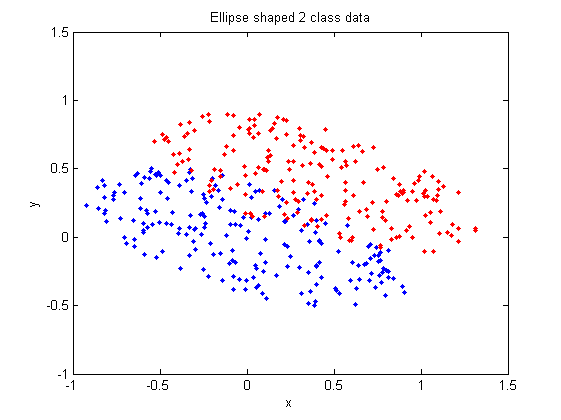
\includegraphics[width=\linewidth]{../Code/Ellipse/svdd/data}
  \caption{2-Ellipse classes dataset with 2 classes}
\end{figure}



The above figure shows a synthetically generated dataset (2-Ellipses) with 2 intersecting ellipses in 2 dimensions.  Clearly, the usage of a spherical decision surface will not be adequate to the separate the points of the 2 classes. To verify this, we plot the decision surfaces obtained on training C-SVDD and F-SVDD on this 2-Ellipses dataset as shown below :

\begin{figure}
\begin{subfigure}{.5\textwidth}
  \centering
  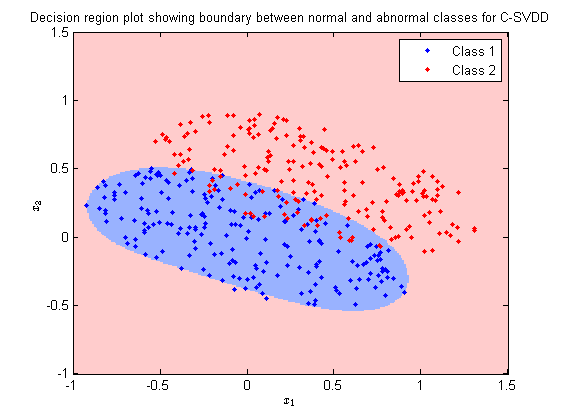
\includegraphics[width=\linewidth]{../Code/Ellipse/svdd/decn}
\caption{C-SVDD} 
\end{subfigure}%
\begin{subfigure}{.5\textwidth}
  \centering
  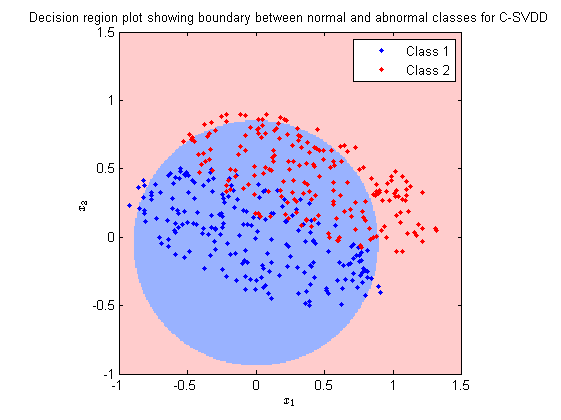
\includegraphics[width=\linewidth]{../Code/Ellipse/fsvdd/decn}
\caption{F-SVDD}  
\end{subfigure}
\caption{Decision region plots obtained on the 2-ellipse dataset}
\end{figure}


As expected , the spherical decision surface constructed by F-SVDD is inadequate to separate the 2 classes but on the contrary, C-SVDD constructs a very good decision elliptical decision surface. This is one of the limitations of F-SVDD in spite it's superior classification speed. But, this problem could be solved by using a different normalized kernel function instead of gaussian. But, as we do not know about the data distribution at hand, it becomes quite challenging.


%\begin{table}[t]
%\caption{Sample table title}
%\label{sample-table}
%\begin{center}
%\begin{tabular}{ll}
%\multicolumn{1}{c}{\bf PART}  &\multicolumn{1}{c}{\bf DESCRIPTION}
%\\ \hline \\
%Dendrite         &Input terminal \\
%Axon             &Output terminal \\
%Soma             &Cell body (contains cell nucleus) \\
%\end{tabular}
%\end{center}
%\end{table}





\subsubsection*{References}

\small{
[1] Tax, David MJ, and Robert PW Duin. "Support vector data description." Machine learning 54.1 (2004): 45-66. 

[2] Liu, Yi-Hung, Yan-Chen Liu, and Yen-Jen Chen. "Fast support vector data descriptions for novelty detection." Neural Networks, IEEE Transactions on 21.8 (2010): 1296-1313.

[3] Hornik, Kurt, Maxwell Stinchcombe, and Halbert White. "Multilayer feedforward networks are universal approximators." Neural networks 2.5 (1989): 359-366.
}

\end{document}